\documentclass{article}
\usepackage{svg}
\usepackage[page]{totalcount} % get \totalpages
\usepackage[perpage]{footmisc} % reset footnote counter at each page
\usepackage{caption} % to use \captionsetup → displays only caption
\usepackage{sidecap} % side captions
\usepackage{listings} % code snippets
\usepackage{amsmath}
\usepackage{amssymb}
\usepackage{pgfplots}
\pgfplotsset{compat=1.18, width=10cm}
\usepackage{algpseudocode}
\usepackage{algorithm}
\usepackage{listings}
\lstdefinelanguage{ASM}{
    morekeywords={mvw, out, add, dec,
        jnz, halt, a, b, c, d},
    morecomment=[l]{;}
}
\lstdefinestyle{mystyle}{
    basicstyle=\ttfamily\footnotesize,   
    breaklines=true,                 
    captionpos=b,                    
    keepspaces=true,                 
    numbers=left,                    
    numbersep=5pt,                  
    showspaces=false,                
    showstringspaces=false,
    showtabs=false,                  
    tabsize=2
}
\lstset{style=mystyle}

\usepackage[sorting=none]{biblatex}
\addbibresource{bibliography.bib}
\usepackage[
  top=2cm,
  bottom=2cm,
  left=2cm,
  right=2cm,
  headheight=17pt, % as per the warning by fancyhdr
  includehead,includefoot,
  heightrounded, % to avoid spurious underfull messages
]{geometry} 
\lstdefinestyle{mystyle}{
    basicstyle=\ttfamily\footnotesize\bfseries,
    breakatwhitespace=false,         
    breaklines=true,                 
    captionpos=t,                    
    keepspaces=true,                 
    numbers=left,                    
    numbersep=5pt,                  
    showspaces=false,                
    showstringspaces=false,
    showtabs=false,                  
    tabsize=2
}% -- Setting up the custom style:
\lstset{style=mystyle}
\usepackage{fancyhdr}
\renewcommand*\contentsname{Table des matières} %"Contents" → "Table des matières"
\renewcommand{\headrulewidth}{0pt} % remove top line in header
\begin{document}
\begin{titlepage}
\begin{center}
    \LARGE
    Gymnase de Renens
    \vspace{2cm} \ \\
    Travail de maturité 2024
    \vspace{5cm} \ \\
    \Huge
    \textbf{Conception et programmation d'un ordinateur 8 bits}
\end{center}
\Large
\vspace{5cm} \ \\
Supervisé par Micha Hersch
\hfill
Écrit par Lukan Morel
\vspace{2cm} \ \\
Renens, 7 novembre 2024
\end{titlepage}
\pagebreak
\markboth{Conception et programmation d'un ordinateur 8 bits}{}
\pagestyle{fancy}
\lhead{Conception et programmation d'un ordinateur 8 bits}
\rhead{\thepage...\totalpages}
\cfoot{}
\tableofcontents
\newpage
\section{Introduction}
Dans notre monde de plus en plus digitalisé, l'on a trop souvent tendance à traiter les ordinateurs comme des boîtes noires auxquelles l'on peut faire aveuglement confiance. Cette confiance est le fruit du travail de nombreux.ses mathématicien.es qui remontent jusqu'à l'Antiquité. En effet, les méthodes pour résoudre des problèmes de manière numérique plutôt que symbolique nous intéressent depuis fort longtemps. Ces méthodes, qu'on regroupe sous le domaine mathématique de l'analyse numérique, se sont faites plus récemment appropriées par les ordinateurs. Avec une importance moindre apportée à l'exactitude mais un intérêt grandissant pour la vitesse, les machines sont bien plus adaptées à ces taches que les humains.
Ce travail a pour objectif de démystifier les opérations internes d'un ordinateur.
Nous y introduirons abstraitement la notion de processeur sans traiter des composants spécifiques à l'implémentation physique d'une telle machine. 
Puis nous montrerons comment, en partant d'opérations basiques et en se servant de l'abstraction comme échelon, nous pouvons atteindre de très grands sommets de complexité mathématique. Sans les résultats présentés dans ce travail, le monde moderne serait tout simplement impossible. L'entièreté de l'informatique, et donc par dépendance, de notre monde est construite sur les concepts fondamentaux que nous verrons ensemble ici. Notons que ce travail aura un accent particulier sur la compréhension et l'intuition plutôt que sur la rigueur. Laissons la rigueur aux artistes qui nous offrent ces résultats dont on profite si volontiers.
Ces sommets mathématiques étant, malgré leur élégance, très accessibles, un grand bagage de connaissances n'est pas nécessaire. Il s'agirait tout de même d'être familier avec quelques notions basiques d'analyse tel que la dérivation et les propriétés des fonctions trigonométriques et logarithmiques. Les autres résultats seront expliqués intuitivement avec plus ou moins de rigueur, en fonction de l'impact sur le niveau de compréhension. Les démarches complètes seront, bien évidemment, référencées dans la bibliographie.
\section{Architecture de la machine}
\subsection{Introduction à l'architecture de CPU}
L'objectif de cette section est de concevoir une machine (qu'on appellera processeur), certes théorique mais tout à fait réaliste, qui sait effectuer un programme informatique. Un programme informatique est une suite d'instructions simples, stockée dans la mémoire externe, qui ensemble, permettent d'exécuter un algorithme bien plus complexe. L'ensemble des instructions est appelé le jeu d'instructions. De par sa taille et complexité, le jeu d'instructions définit les capacités du processeur: les ordinateurs d'aujourd'hui ont donc un jeu d'instructions bien plus grand et complexe que celui utilisé ici. Le jeu d'instructions comporte plusieurs types d'instructions que l'on peut classer en trois grandes familles: les instructions logiques et arithmétiques, les instructions de gestion de mémoire et les instructions de contrôle d'exécution.
Les instructions logiques et arithmétiques permettent au processeur d'effectuer des opérations mathématiques. Il est important de noter que ces instructions n'opèrent pas directement sur les données stockées en mémoire externe. Au lieu de cela, les valeurs nécessaires sont transférées depuis la mémoire externe vers la mémoire interne du processeur (appelée les registres), sur laquelle on peut opérer. Puis, une fois les opérations terminées, les valeurs sont renvoyées dans la mémoire externe. Ceci est dû au fait que l'accès à la mémoire externe est bien plus lent que celui à la mémoire interne. Mais là où la mémoire interne gagne en vitesse, elle s'écrase lamentablement pour ce qui est de la taille. Ce compromis soulève alors un besoin pour des instructions dédiées aux transferts entre la mémoire externe et interne: les instructions de gestion de mémoire. Finalement, les instructions de contrôle d'exécution proposent une alternative à l'exécution linéaire des instructions. En effet, elles permettent de faire déplacer l'exécution vers une autre partie du programme. Ce déplacement est appelé un branchement. Un branchement devient particulièrement utile lorsqu'il est soumis à une condition. La valeur de vérité d'une proposition mathématique qui implique, ou non, un branchement permet au programme de prendre des décisions sur la suite de l'exécution en fonction du début. Ces branchements conditionnels sont un concept capital pour tout programme informatique. Armé d'un jeu d'instructions qui comporte au minimum ces trois types d'instructions et d'un processeur qui sait les exécuter, l'on a ce que celles et ceux qui l'ont conçu avant nous ont appelé, un CPU (Central Processing Unit). Les prochaines sous-sections auront pour but d'expliquer plus en détail les différents composants du processeur et de décrire le jeu d'instructions sur lequel nous allons travailler.
\pagebreak

\subsection{RAM}
La RAM (Random Access Memory) ou mémoire externe, contient les informations nécessaires à l'exécution d'un programme (code du programme, variables, etc.). Les données sont séparées en blocs de un octet. Chaque octet est assigné une adresse de 16 bits, soit 2 octets, on a donc une mémoire totale de 64 KiB. ($2^{16} = 65536$)
\\Les adresses sont souvent représentées en hexadécimal et sont donc préfixées de “0x”.
\begin{figure}[htp]
    \centering
    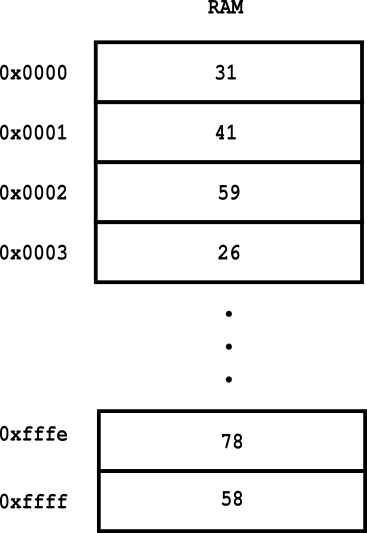
\includegraphics[width=5cm]{images/ram_diagram.png}
    \label{fig:ram}
\end{figure}
\\
Lors de l'exécution d'un programme, le code se trouve au début de la mémoire, puis viennent les données numériques. Le stack se trouve à la fin et grandit en direction du début.
\begin{figure}[htp]
    \centering
    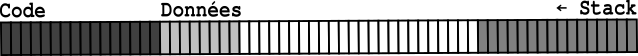
\includegraphics[width=9cm]{images/ram_layout_diagram.png}
    \label{fig:ram_layout}
\end{figure}
\\
\subsection{Stack}
Le stack ou pile, est une structure de données, placée dans la RAM, qui opère sur le principe suivant: dernier rentré, premier sorti. 
\\Nous pouvons l'imaginer comme une pile d'assiettes: l'on peut ajouter et récupérer des assiettes seulement depuis le haut de la pile.
Ces deux opérations sont gérées nativement par les instructions \texttt{push}\footnote{Voir Instructions} et \texttt{pop} respectivement.
\\
L'adresse du haut du stack est stockée, relativement au cadre actuel, dans le registre \texttt{sp}\footnote{Voir Registres}. L'adresse absolue est alors donnée par \texttt{fp} - \texttt{sp}. Le stack sert principalement à stocker les données specifiques à l'appel d'une fonction. 
\subsubsection{Cadre}
Un cadre est un espace de mémoire dans le stack réservé au données spécifiques à l'appel d'une fonction. Quand une fonction est appelée, un nouveau cadre, ainsi que l'addresse de retour, est placé sur le stack. Toutes les variables spécifiques ou locales seront stockées dans le cadre. Une fois la fonction terminée elles seront oubliées et le programme reprendra depuis l'addresse de retour.

\pagebreak

\subsection{Registres}
Un registre est un emplacement de mémoire interne au processeur dont l'accès est très rapide. La plupart des instructions\footnote{Voir Instructions} opèrent directement sur les registres. Il y a 8 registres, de un octet chacun, à notre disposition, listés ci-dessous:
\begin{itemize}
    \item Registre \texttt{a}, registre à usage général.
    \item Registre \texttt{b}, registre à usage général.
    \item Registre \texttt{c}, registre à usage général.
    \item Registre \texttt{d}, registre à usage général.
    \item Registre \texttt{hfp} (High Frame Pointer), stocke le premier octet de l'adresse du cadre actuel.
    \item Registre \texttt{lfp} (Low Frame Pointer), stocke le dernier octet de l'adresse du cadre actuel.
    \item Registre \texttt{sp} (Stack Pointer), stocke l'adresse du haut du stack relativement au cadre actuel.
    \item Registre \texttt{f} (Flag), stocke l'état des huit drapeaux:
    \begin{itemize}
        \item \texttt{positive} (Positif), le résultat de l'opération est positif.
        \item \texttt{carry} (Retenue), l'opération mène à une retenue.
        \item \texttt{equal} (Egal), le registre est égal au registre ou à la valeur à laquelle il est comparé.
        \item \texttt{zero} (Zéro), le résultat l'opération est nul.
        \item \texttt{less} (Moins), le registre est inférieur au registre ou à la valeur à laquelle il est comparé.
        \item \texttt{borrow} (Emprunt), la soustraction mène à un emprunt.
        \item \texttt{negative} (Négatif), le résultat de l'opération est strictement négatif.
        \item \texttt{overflow} (Débordement), le résultat de l'opération ne rentre pas dans un registre.
    \end{itemize}
\end{itemize}
Les drapeaux \texttt{negative} et \texttt{overflow} sont utiles qu'en arithmétique signée, ou les valeurs sont représentées en complément à 2. Étant donné que ces drapeaux ne sont jamais utilisés dans le reste du travail, l'on peut ne pas les considérer.
Les opérations; \texttt{add}, \texttt{sub}, \texttt{adc}, \texttt{sbb}, \texttt{iec}, \texttt{bsl} et \texttt{bsr} provoquent une mise à jour des drapeaux.\\
Les paires de registres (\texttt{a}, \texttt{b}) et (\texttt{c}, \texttt{d}) sont souvent utilisés ensemble et forment alors deux registres de 2 octets chacun nommés \texttt{ab} et \texttt{cd}, respectivement. La valeur de \texttt{ab} est donnée par $\texttt{a}\cdot 256 + \texttt{b}$ et pareillement pour \texttt{cd}.
\begin{figure}[htp]
    \centering
    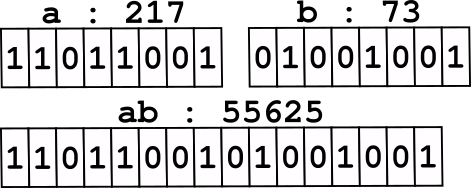
\includegraphics[width=5cm]{images/register_composition.png}
    \label{fig:register_composition}
\end{figure}

\pagebreak

\subsection{Jeu d'instructions}
Le jeu d'instructions regroupe la totalité des opérations que la machine peut effectuer. En combinant ces instructions il est possible d'implémenter n'importe quel algorithme. Ci-dessous sont décrits les 16 instructions natives au processeur.
\begin{itemize}
    \item \texttt{ldw} (Load Word), copie le contenu d'une adresse ou celle décrite par les registres \texttt{ab} ou \texttt{cd} dans un registre.
    \item \texttt{stw} (Store Word), copie le contenu d'un registre dans une adresse ou celle décrite par les registres \texttt{ab} ou \texttt{cd}.
    \item \texttt{mvw} (Move Word), copie le contenu d'un registre ou une valeur immédiate dans un autre registre.
    \item \texttt{add} (Add), additionne le contenu d'un registre ou une valeur immédiate à un autre registre et copie le résultat dans le premier registre.
    \item \texttt{sub} (Subtract), soustrait le contenu d'un registre ou une valeur immédiate à un autre registre et copie le résultat dans le premier registre.
    \item \texttt{adc} (Add with Carry), effectue l'opération \texttt{add} en ajoutant à l'addition la valeur du drapeau \texttt{carry}.
    \item \texttt{sbb} (Subtract with Borrow), effectue l'operation \texttt{sub} en ajoutant à la soustraction la valeur du drapeau \texttt{borrow}.
    \item \texttt{iec} (Increment/Decrement), incrémente ou décrémente de 1 le contenu d'un registre et stocke le résultat dans ce dernier.
    \item \texttt{cmp} (Compare), compare le contenu d'un registre avec le contenu d'un autre ou d'une valeur immédiate et met à jour les drapeaux appropriés.
    \item \texttt{jnz} (Jump if Not Zero), effectue un branchement vers une adresse ou celle décrite par le registre \texttt{ab} ou \texttt{cd} si le drapeau \texttt{zero} n'est pas activé.
    \item \texttt{push} (Push), copie le contenu d'un registre ou celui d'une adresse en haut de la pile et incrémente de 1 le contenu du registre \texttt{sp}.
    \item \texttt{pop} (Pop), copie le contenu du haut de la pile dans un registre ou une adresse et décrémente de 1 le contenu du registre \texttt{sp}.
    \item \texttt{bsl} (Bit Shift Left), décale vers la gauche les bits d'un registre ou des registres \texttt{ab} ou \texttt{cd} et copie le résultat dans ce(s) dernier(s).
    \item \texttt{bsr} (Bit Shift Right), décale vers la droite les bits d'un registre ou des registres \texttt{ab} ou \texttt{cd} et copie le résultat dans ce(s) dernier(s).
    \item \texttt{out} (Out), affiche le contenu d'un registre comme une valeur absolue ou comme une valeur en complément à 2.
    \item \texttt{halt} (Halt), halte l'éxécution du programme.
\end{itemize}
Un programme est constitué d'une séquence de ces instructions. Mais puisque la RAM qui contient le programme ne peut que stocker des nombres sous forme de bytes, chaque instruction doit être traduite en un nombre unique qui sera lui stocké. De cette manière, le processeur pourra comprendre les programmes qu'on lui donne. Ce processus de traduction s'appelle l'assemblage.
\newpage
\subsection{Assemblage}
L'assemblage se charge de traduire le fichier textuel d'un programme en un fichier binaire qui pourra être chargé dans la RAM du processeur afin d’effectuer le programme en question. \cite{salomon1992assemblers} Chaque ligne de code, à l'exception des commentaires et des définitions, est alors traduite de cette manière; puisqu'il y a 16 instructions, on dédie 4 bits pour encoder l'instruction en question. Ensuite, on dédie un bit pour encoder le réglage spécifique de l'instruction. Par exemple pour l'instruction $\texttt{add}$, l'on peut soit additionner un registre à un autre ($\texttt{add a, b}$), soit additionner un registre à une valeur immédiate ($\texttt{add a, 42}$). Le 5-ième bit choisit alors entre ces possibilités. Il nous reste donc, dans un byte, 3 bits avec lesquels on spécifie le registre sur lequel l'instruction à effet. On utilise le ou les byte(s) d'après pour spécifier un deuxième registre, une valeur immédiate, ou une adresse immédiate. Essayons alors d'assembler la ligne de code $\texttt{add a, b}$.\\ $\texttt{add}$ est la 3-ième instruction en partant de 0. Les premiers 4 bits seront alors 0011. On désire additionner deux registres, alors le bit de réglage est 0. Le registre $\texttt{a}$ est le premier, alors les 3 prochains bits sont 000. Finalement le registre $\texttt{b}$ est le deuxième donc le prochain byte est 00000001. Le code traduit est alors 00110000 00000001. Soit, cette ligne de code, une fois assemblée, tiens sur deux bytes. Les ligne de codes assemblées peuvent varier en longueur de un à trois bytes.

\subsection{Exemple de programme}
Mettons maintenant en œuvre ces instructions.
Voyons un exemple de programme que notre machine peut effectuer. Il s'agit ici de calculer un certain nombre de termes de la suite de Fibonacci. Notons pour rappel que la suite de Fibonacci $(F_n)_{n\in\mathbb{N}}$ est définie comme tel:
$$
\begin{cases}
F_0 = 0\\
F_1 = 1\\
F_n = F_{n-1} + F_{n-2}\\
\end{cases}
$$
Voici alors le programme:
\begin{figure}[htp]
    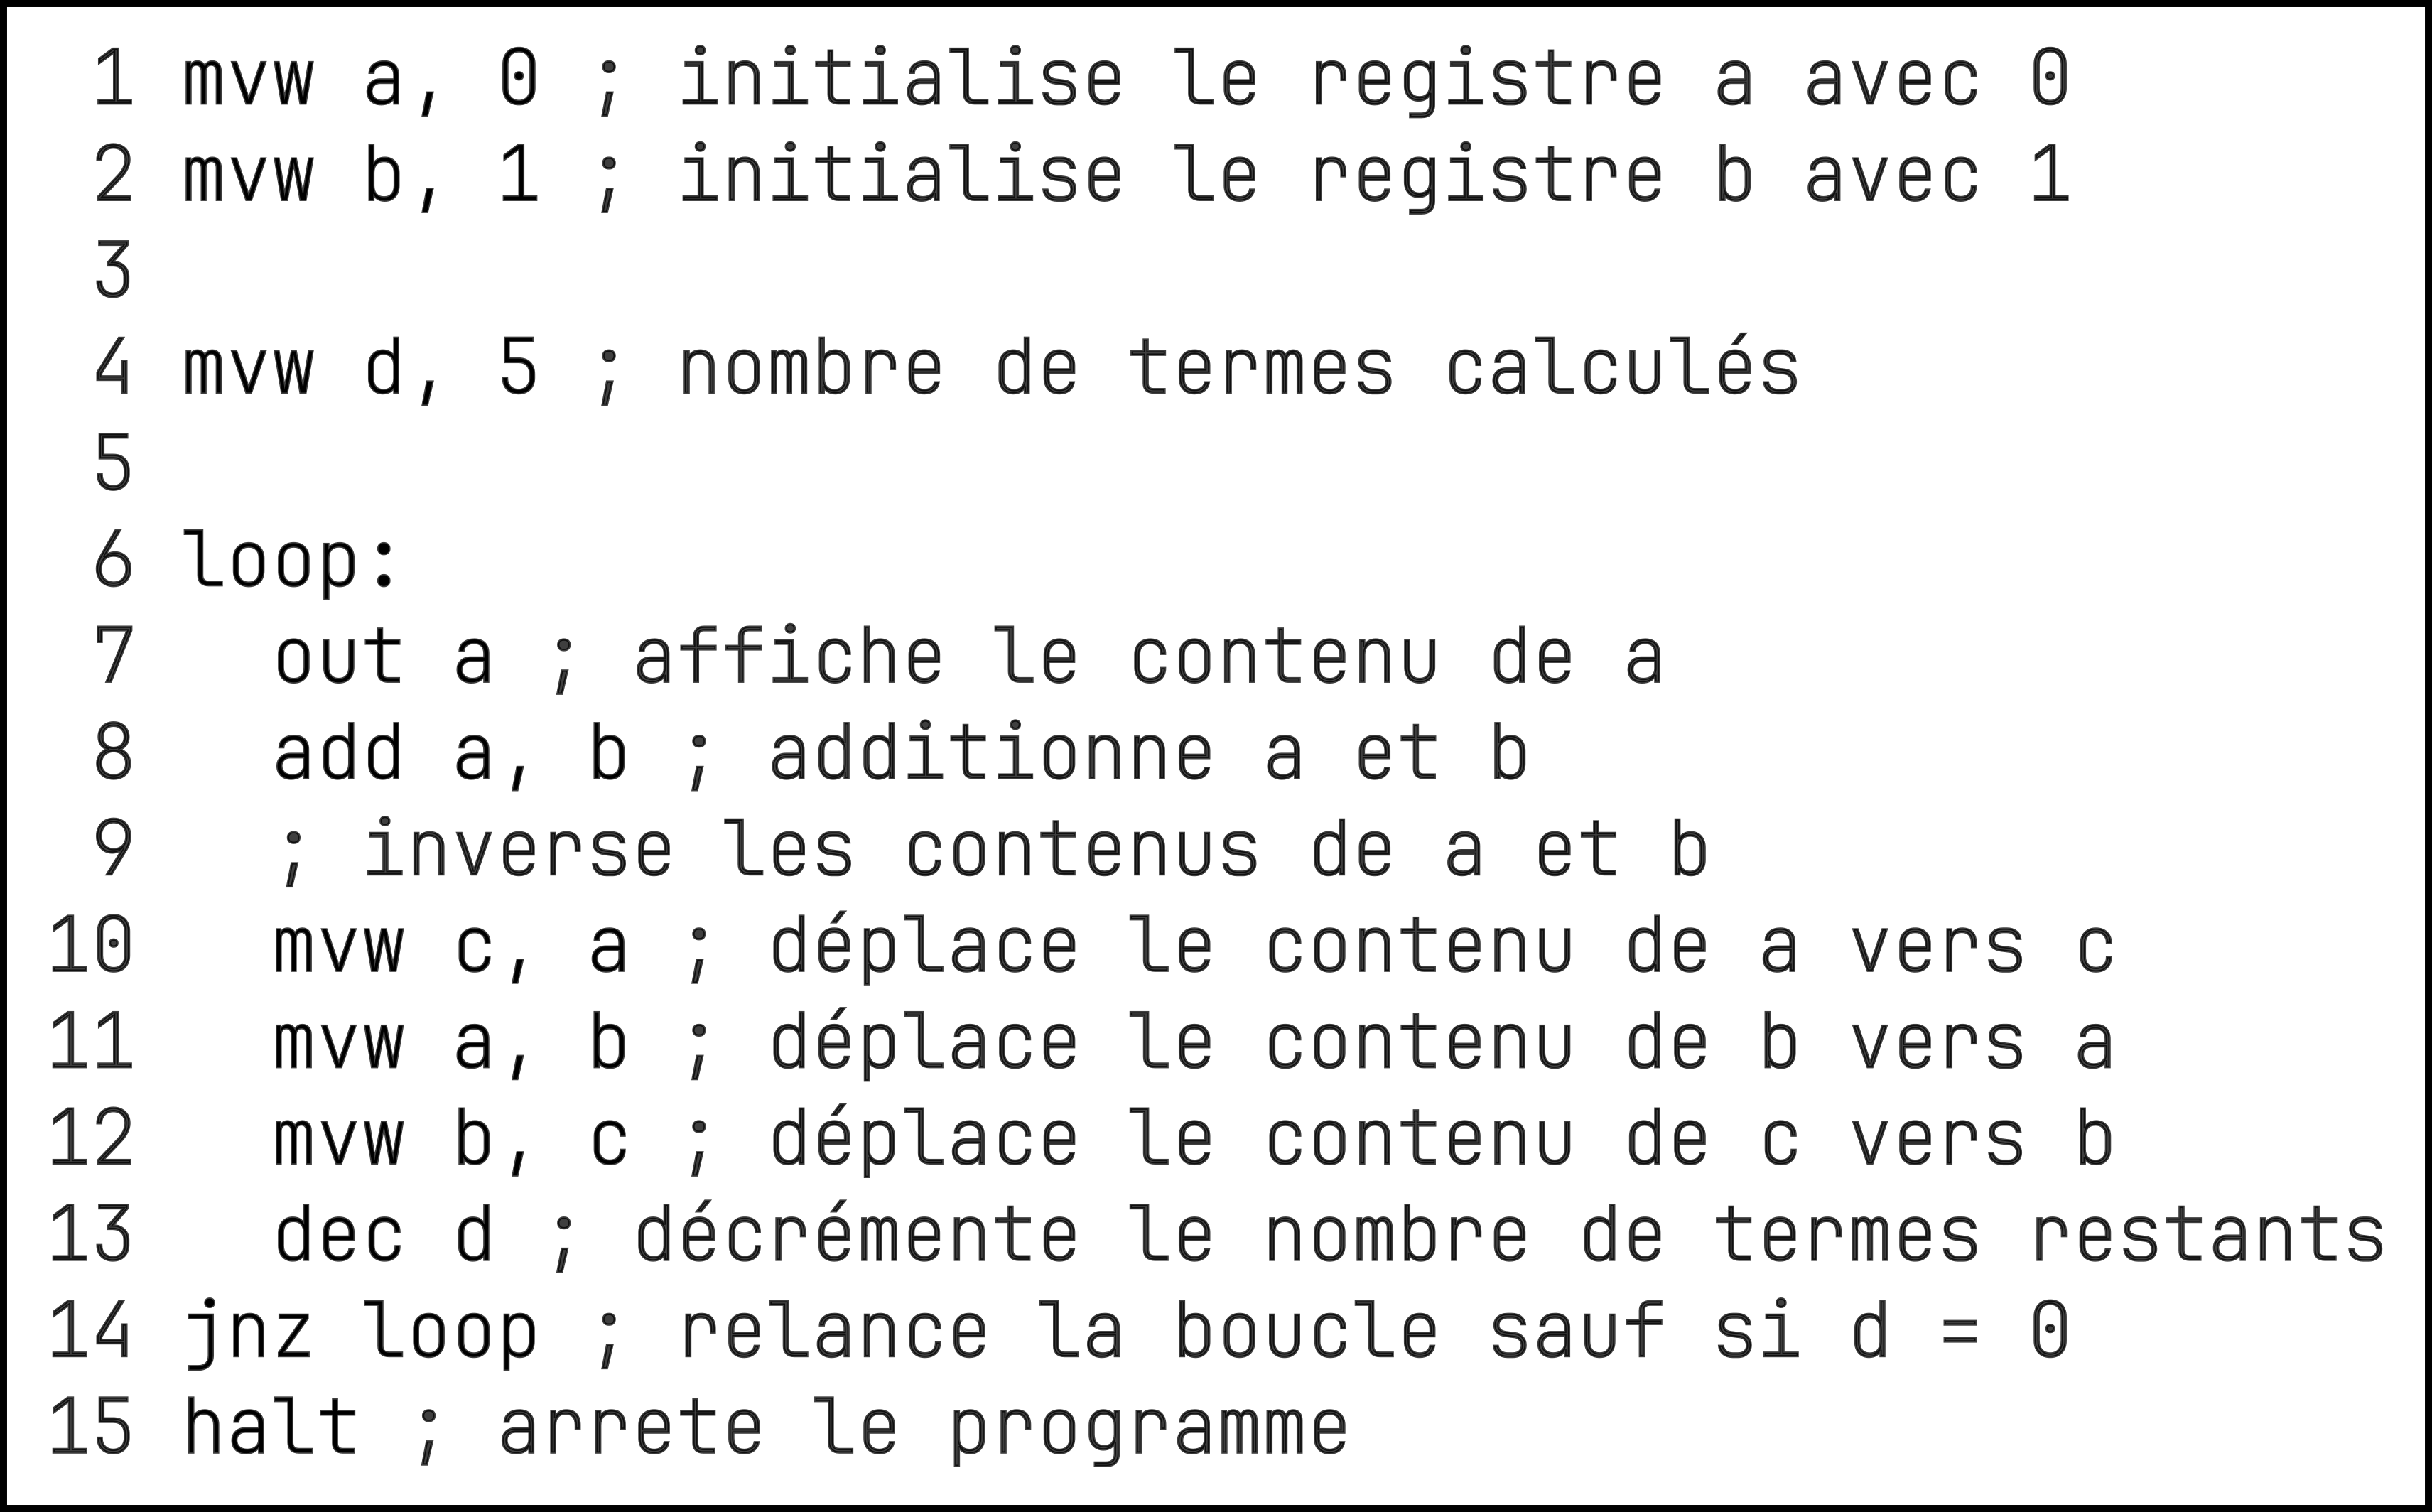
\includegraphics[width=10cm]{images/program.png}
    \label{fig:program}
\end{figure}
\\
Ce programme, une fois assemblé et exécuté par le processeur, affichera à la console: 0, 1, 1, 2, 3. Soit les 5 premiers termes de la suite de Fibonacci.
Ici, la valeur de 5 est choisie arbitrairement. Le programme aurait pu calculer jusqu'à n'importe quel terme, tant que ce terme n'excède pas 255. Dans quel cas les résultats affichés seraient réduits modulo 256. Pour exécuter un tel programme on utilise un émulateur. L'émulateur prend en entrée un programme assemblé et effectue un par un chaque instruction en utilisant une RAM et des registres simulés. C'est donc équivalent à faire tourner le programme sur une vraie machine physique. Dans la prochaine section nous traiterons en détail plus spécifiquement des instructions arithmétiques et leurs impacts sur le registre des drapeaux.
\section{Opérations sur entiers}
\subsection{Addition}
L'addition est une opération native au processeur, gérée par les instructions \texttt{add} et \texttt{adc}.
L'instruction est utilisée comme-tel:\\

\begin{center}
\texttt{add x, y}
\end{center}
avec \texttt{x} un registre et \texttt{y} un registre ou une valeur immédiate.\\Alors le résultat de l'opération sera stocké dans le registre \texttt{x}. Il est important de noter que puisque le registre ne peut que stocker des valeurs allant jusqu'à 255, le résultat de l'opération sera modulo 256.
Soit, 
$$\texttt{add x, y} \implies \texttt{x} \leftarrow \texttt{x} + \texttt{y} \mod 256$$
Si le résultat de \texttt{x} + \texttt{y} dépasse 255, alors le drapeau \texttt{carry} sera activé. On peut donc le considérer comme le neuvième bit du résultat. Son activation est décrite par,
$$\texttt{add x, y} \implies \texttt{carry} = \begin{cases}
1, & \texttt{x} + \texttt{y} > 255\\
0, & \text{sinon.}
\end{cases}$$
Si le résultat de \texttt{x} + \texttt{y} est nul, alors le drapeau \texttt{zero} sera activé. Son activation est décrite par,
$$\texttt{add x, y} \implies \texttt{zero} = \begin{cases}
1, & \texttt{x} + \texttt{y}\mod 256= 0\\
0, & \text{sinon.}
\end{cases}$$
L'instruction \texttt{adc} fonctionne pareillement à \texttt{add} mais elle additionne en plus la valeur du drapeau \texttt{carry}.
\subsection{Soustraction}
La soustraction est une opération native au processeur, gérée par les instructions \texttt{sub} et \texttt{sbb}. L'instruction est utilisée comme-tel:
\begin{center}
\texttt{sub x, y}
\end{center}
avec \texttt{x} un registre et \texttt{y} un registre ou une valeur immédiate.\\
Alors le résultat de l'opération sera stocké dans le registre \texttt{x}. Comme pour l'addition le résultat est modulo 256, ce qui permet de gèrer les résultats négatifs. Soit,
$$\texttt{sub x, y} \implies \texttt{x} \leftarrow \texttt{x} - \texttt{y} \mod 256$$
Pour indiquer un résultat négatif, le drapeau \texttt{borrow} est activé. Son activation est décrite par,
$$\texttt{sub x, y} \implies \texttt{borrow} = \begin{cases}
1, & \texttt{x} - \texttt{y} < 0\\
0, & \text{sinon.}
\end{cases}$$
Si le résultat de \texttt{x} - \texttt{y} est nul, alors le drapeau \texttt{zero} sera activé. Son activation est décrite par,
$$\texttt{sub x, y} \implies \texttt{zero} = \begin{cases}
1, & \texttt{x} - \texttt{y}\mod 256= 0\\
0, & \text{sinon.}
\end{cases}$$
L'instruction \texttt{sbb} fonctionne pareillement à \texttt{sub} mais elle soustrait en plus la valeur du drapeau \texttt{borrow}.
\subsection{Décalage de bits}
Le décalage de bits est une opération native au processeur, gérée par les instructions \texttt{bsl} et \texttt{bsr}. L'instruction est utilisée comme-tel:
\begin{center}
\texttt{bsl x}
\end{center}
avec x un registre.
Alors le résultat sera stocké dans le registre \texttt{x}. Le décalage de bits consiste à décaler les bits d'une valeur vers la gauche ou vers la droite.
L'opération est notée \texttt{x}\verb| << |1 pour un décalage vers la gauche ou \texttt{x}\verb| >> |1 pour un décalage vers la droite.
L'on peut considérer ces opérations comme une multiplication par deux et une division à partie entière par deux respectivement. Soit, 
\begin{align*}
&\texttt{bsl x} \implies \texttt{x} \leftarrow2\texttt{x}\mod 256\\
&\texttt{bsr x} \implies \texttt{x} \leftarrow \left\lfloor\frac{\texttt{x}}{2}\right\rfloor
\end{align*}

Si, après un décalage, un bit a été déplacé hors du registre, que ce soit vers la gauche ou la droite, le drapeau \texttt{carry} sera activé comme-tel:
$$\texttt{bsl x} \implies \texttt{carry} = \begin{cases}
1, & \texttt{x}\verb| << | 1 > 255\\
0, & \text{sinon.}
\end{cases}$$
$$\texttt{bsr x} \implies \texttt{carry} = \begin{cases}
1, & \texttt{x}\verb| >> | 1 < \frac{\texttt{x}}{2}\\
0, & \text{sinon.}
\end{cases}$$

Si le résultat d'un décalage est nul, alors le drapeau \texttt{zero} sera activé. Son activation est décrite par,
$$\texttt{bsl x} \implies \texttt{zero} = \begin{cases}
1, & \texttt{x}\verb| << | 1 = 0\\
0, & \text{sinon.}
\end{cases}$$
$$\texttt{bsr x} \implies \texttt{zero} = \begin{cases}
1, & \texttt{x}\verb| >> | 1 = 0\\
0, & \text{sinon.}
\end{cases}$$
Il est également possible de décaler deux registres ensemble comme si ils n'étaient qu'un avec \texttt{bsl ab}, \texttt{bsl cd} et \texttt{bsr ab}, \texttt{bsr cd}.
\subsection{Multiplication}
Dans le reste du travail, la multiplication d'entiers sera occasionnellement utile. On distingue alors deux cas de figure.
Celui ou l'on veut multiplier une variable par une constante et celui ou l'on veut multiplier une variable par une autre variable.
Pour le premier cas on alors l'opération $x\cdot c$, ou $c$ est une constante. En réécrivant $c$ comme une somme de puissances de 2 on a
$$
x\cdot(a_02^0+a_12^1+\cdot\cdot\cdot+a_72^7) \text{, avec $a_k$ = 1 ou 0.}
$$
On distribue pour obtenir
$$x\cdot a_02^0+x\cdot a_12^1+\cdot\cdot\cdot+x\cdot a_72^7.$$
Et puisque $x\cdot2^n$ est égal à $n$ décalages de $x$ vers la gauche, 
le problème est résolu. Par exemple, multiplier $x$ par 10 revient à évaluer $x$\verb|<<|1 + $x$\verb|<<|3.\\
Le deuxième cas est plus complexe. La multiplication par additions répétées,
$$
x\cdot y = \underbrace{x+x+\cdot\cdot\cdot+x}_{y\text{ fois}},
$$
est souvent découragée car elle devient beaucoup moins efficace que d'autres méthodes plus sophistiquées quand les facteurs deviennent de plus en plus grand. Mais étant donné que nous travaillons sur des valeurs plutôt petites, la simplicité offerte par cette méthode naïve en vaut la peine. C'est alors par additions répétées que nous procéderons.
\section{Opérations sur nombres non entiers}
Afin de répondre à un plus grand nombre de problèmes mathématiques il sera utile de travailler non pas que sur des entiers mais également sur les rationaux qui les entourent. Il s'agit donc de définir une représentation et des opérations élémentaires pour ces valeurs fractionnelles.
\subsection{Représentation à virgule flottante}
Le standard utilisé universellement pour représenter des valeurs fractionnelles dans les ordinateurs est celui de la virgule flottante (ou floating point en anglais). Les valeurs de ce type sont appelées des floats. Un float est composé de trois parties:
\begin{itemize}
    \item un signe, $s\in \{-1, 1\}$;
    \item un exposant, $E$;
    \item une mantisse, $M$.
\end{itemize}
Ces trois parties sont telles que la valeur du float est donnée par $s\cdot M\cdot 2^E$.\\
Ce système s'apparente à être l'équivalent de la notation scientifique pour le binaire.
Il reste maintenant la question de comment encoder ces trois parties dans un espace fini et compact. Nous allons choisir comme taille 16 bits. L'encodage du signe $s$ est intuitif, nous pouvons y dédier le premier bit (0 si $s$ = 1, 1 si $s$ = -1). La taille de l'exposant déterminera l'ordre de grandeur minimal et maximal de nos floats. Si l'on attribue 5 bits à l'exposant, ce dernier peut avoir $2^5 = 32$ valeurs différentes. Étant donné qu'il nous faut aussi des exposants négatifs nous pouvons ajouter un biais à l'exposant. C'est-à-dire que l'exposant $E = E_s - 15$ où $E_s$ est l'entier véritablement représenté par les 5 bits dédiés. Les valeurs sont donc bornées par $2^{-15}$ et $2^{16}$. Il nous reste alors 10 bits pour la mantisse.
Notons que, comme en notation scientifique, la mantisse $M$ doit pouvoir représenter des valeurs non entières dans l'intervalle $[1; 2[$. Notons ensuite que toutes les valeurs incluses dans cet intervalle ont comme partie entière 1. Puisque la partie entière est constante, il n'est pas nécessaire de la stocker. Soit, la mantisse $M = 1+2^{-10}M_s)$ où $M_s$ est l'entier véritablement stocké par les 10 bits dédiés. Finalement, la valeur d'un float est donnée par
$$(-1)^{s_s}\left(1+\frac{M_s}{2^{10}}\right)\cdot 2^{E_s-15},\text{ ou $s_s$ est la valeur du premier bit.}$$
Cette formule n'est pas générale, dans certain cas spéciaux le float doit être interprété différemment. Ceci est nécessaire pour représenter des valeurs comme 0 ou $\pm\infty$.
Plus généralement la valeur d'un float est donnée par
$$\begin{cases}
(-1)^{s_s}(1+\frac{M_s}{2^{10}})\cdot 2^{E_s-15}, & E_s \not\in \{0,31\}\\
(-1)^{s_s}\frac{M_s}{2^{10}}\cdot 2^{E_s-15}, & E_s = 0 \text{ et } M_s \not=0\\
0, & s_s = 0,\,E_s = 0 \text{ et } M_s=0\\
-0, & s_s = 1,\,E_s = 0 \text{ et } M_s=0\\
+\infty, & s_s = 0,\,E_s = 31 \text{ et } M_s=0\\
-\infty, & s_s = 1,\,E_s = 31 \text{ et } M_s=0\\
\text{NaN}, & E_s = 31 \text{ et } M_s\not=0\\
\end{cases}$$
NaN (Not a Number), désigne une valeur indéterminée comme par exemple le résultat de $\frac{0}{0}$.\\
\newpage
En mémoire un float est disposé comme tel
\begin{figure}[htp]
    \centering
    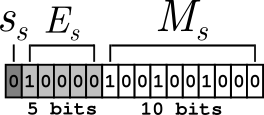
\includegraphics[width=5cm]{images/float16.png}
    \label{fig:float16}
\end{figure}\\
$$(-1)^{s_s}\left(1+\frac{M_s}{2^{10}}\right)\cdot 2^{E_s-15} = (-1)^{0}\left(1+\frac{584}{2^{10}}\right)\cdot 2^{16-15}=1.57\cdot 2 = 3.14$$
Il s'agit maintenant de définir des procédures pour opérer sur ces floats.
\subsection{Addition et soustraction de floats}
Pour additionner deux floats $\alpha$ et $\beta$ en un float $\Gamma$, il faut premièrement extraire les signes, exposants et mantisses des floats $\alpha$ et $\beta$. Ensuite, en établissant la relation suivante
$$s_{\Gamma}\cdot M_{\Gamma} \cdot 2^{E_{\Gamma}} = s_{\alpha}\cdot M_{\alpha} \cdot 2^{E_{\alpha}}+s_{\beta}\cdot M_{\beta} \cdot 2^{E_{\beta}}$$
on remarque que si $E_{\alpha} = E_{\beta}$, le problème devient trivial. Il suffit d'abord de convertir les mantisses de $\alpha$ et $\beta$ en complément à 2 en fonction du signe, puis de les additionner. Si le résultat de l'addition de mantisses est négatif il faudra reconvertir le résultat du complément à 2 et $s_{\Gamma} = -1$. Finalement on décale les bits du résultat de sorte à ce que la partie entière soie 1 et on change l'exposant en conséquence. Le résultat et l'exposant normalisés nous donnent $M_{\Gamma}$ et $E_{\Gamma}$ respectivement. Le cas $E_{\alpha} \not= E_{\beta}$ ajoute une étape avant l'addition des mantisses. Il faut d'abord décaler les bits de la mantisse du plus petit nombre $|E_{\alpha}-E_{\beta}|$ fois vers la droite.

La soustraction de floats suit le même processus que l'addition, à l'exception que l'addition de mantisses est substituée, sans surprise, par une soustraction. Dans le cas ou le résultat dépasse les bornes de notre représentation, l'on peut simplement retourner plus ou moins l'infini.
\subsection{Multiplication de floats}
Pour multiplier deux floats $\alpha$ et $\beta$ en un float $\Gamma$, il faut premièrement extraire les signes, exposants et mantisses des floats $\alpha$ et $\beta$. Ensuite, en établissant la relation suivante
\begin{align*}
    s_{\Gamma}\cdot M_{\Gamma} \cdot 2^{E_{\Gamma}} &= s_{\alpha}\cdot M_{\alpha} \cdot 2^{E_{\alpha}}\,\cdot\,s_{\beta}\cdot M_{\beta} \cdot 2^{E_{\beta}}\\
    &= s_{\alpha}s_{\beta}\cdot M_{\alpha}M_{\beta}\cdot 2^{E_{\alpha}+E_{\beta}}
\end{align*}
on remarque qu'il suffit de multiplier les signes, les mantisses et d'additionner les exposants, puis de normaliser le résultat pour obtenir $\Gamma$. Dans le cas ou le résultat dépasse les bornes de notre représentation, l'on peut simplement retourner plus ou moins l'infini.
\subsection{Division de floats}
Pour diviser deux floats nous allons multiplier l'un par l'inverse de l'autre. Nous détaillerons ci-dessous une manière très efficace de trouver une approximation de la réciproque d'un float. Cette approximation pourra ensuite être améliorée avec quelques itérations de la méthode de Newton.
\subsubsection{La méthode de Newton}
La méthode de Newton est un algorithme efficace pour trouver numériquement les zéros d'une fonction. Afin de la comprendre, admettons que nous essayons de trouver un zéro de la fonction $f(x) = x^2-1$. Nous avons une estimation initiale $x_0 = 3$. C'est à dire que nous pensons que le zéro cherché n'est pas trop loin de 3. En traçant la tangente à la courbe $f(x)$ en $x_0$, on s'aperçoit que le croisement entre cette tangente et l'axe des abscisses nous donne une meilleure estimation du zéro de la fonction. En procédant itérativement, on s'approche de plus en plus du zéro.
\begin{center}
\begin{tikzpicture}
\begin{axis}[xmin=0, xmax=3, ymin=-2, ymax=8,
             axis lines=middle,
             xtick={1, 2, 3, 4},
             xticklabels={1, 2, 3, 4},
             ytick={-2, 0.004 , 2, 4, 6, 8},
             yticklabels={-2, 0, 2, 4, 6, 8},
             xticklabel style={anchor=north},
             legend pos=south east
             ]
\addplot[thick, domain=0:3, color=black, samples=100] {x^2-1} node [left, pos=0.9] {$f(x)$};
\addplot[thick, domain=5/3:3, dashed, color=black = 10] {6*x-10};
\addplot[color = black, mark = *, only marks, mark size = 1pt] coordinates {(3, 0) (3, 8) (5/3, 0) (5/3, 16/9) (17/15, 0)};
\addplot[thick, domain=17/15:5/3, dashed, color=black = 10] {16/9+(10/3)*(x-5/3)};
\addplot[color = black, densely dashed,] coordinates {(3, 0) (3,8)};
\addplot[color = black, densely dashed,] coordinates {(5/3, 0) (5/3,16/9)};
\node [above left] at (3, 0) {$x_0$};
\node [below] at (5/3, 0) {$x_1$};
\node [below] at (17/15, 0) {$x_2$};
\end{axis}
\end{tikzpicture}
\end{center}
La tangente à $f(x)$ en $x_0$ est donnée par $f(x_0)+f'(x_0)(x-x_0)$. Alors $f(x_0)+f'(x_0)(x_1-x_0) = 0$.
En isolant $x_1$, on trouve
$$
x_1 = x_0-\frac{f(x_0)}{f'(x_0)}.
$$
Et plus généralement
$$
x_{n+1} = x_n-\frac{f(x_n)}{f'(x_n)}.
$$
Notons que dans certains cas, la méthode ne parviendra pas à converger vers le zéro désiré. Par exemple dans le cas trivial où $f'(x_n) = 0$ mais $f(x_n) \not = 0$. Dans ce cas la division par $f'(x_n)$ n'est pas définie. Graphiquement, la tangente est parallèle à l'axe des abscisses et donc ne la croise jamais. Une autre raison d'échec potentiel serait que la méthode converge vers un zéro non désiré. Ceci arrive si l'on choisit un $x_0$ trop loin du zéro désiré.
\subsubsection{Approximation de la réciproque}
Pour calculer la réciproque d'un float, notons d'abord qu'un float $\alpha$ est un nombre de 16 bits que l'on interprète comme un float. Dans quel cas, la valeur de $\alpha$, qu'on appelle $\alpha_f$ est donnée par
$$\alpha_f=\left(1+\frac{M_{s,\alpha}}{2^{10}}\right)\cdot 2^{E_{s,\alpha}-15}.\,\footnote{Le signe n'est pas pris en compte, on admet que le float est positif. Dans le cas contraire, il suffit de multiplier par -1 le résultat obtenu.}$$\\
Mais si l'on interprète $\alpha$ comme un entier, sa valeur $\alpha_i$ (appelée représentation entière de $\alpha$) est donnée par
$$\alpha_i=2^{10}E_{s, \alpha} + M_{s, \alpha}.$$
En sachant ceci, prenons maintenant le logarithme base 2 de $\alpha_f$
\begin{align*}
    \log_2(\alpha_f)&=\log_2\left(\left(1+\frac{M_{s,\alpha}}{2^{10}}\right)\cdot 2^{E_{s,\alpha}-15}\right)\\
    &=\log_2\left(1+\frac{M_{s,\alpha}}{2^{10}}\right)+E_{s,\alpha}-15\\
    \intertext{Remplaçons maintenant le premier terme par une approximation pour $\log_2(1+x)$, soit $x + \mu$ où $\mu$ est tel qu'il minimise $\max_{0\le x\le 1}|\log_2(1+x) - (x + \mu)|$}\\
    &\approx\frac{M_{s,\alpha}}{2^{10}}+\mu+E_{s,\alpha}-15\\
    &\approx\frac{1}{2^{10}}(2^{10}E_{s, \alpha} + M_{s, \alpha})+\mu-15\\
    \log_2(\alpha_f)&\approx\frac{1}{2^{10}}(\alpha_i)+\mu-15.\\
\end{align*}
Cette relation nous dit que le logarithme base 2 d'un float est directement lié à son entier associé, ce qui s’avérera être très utile par la suite. Néanmoins il s'agirait de clarifier l'approximation $\log_2(1+x) \approx x+\mu$ et de déterminer comment trouver une valeur numérique pour $\mu$. On cherche donc un polynôme $p(x) = \lambda x + \mu$, tel qu'il soit le polynôme de degré 1 qui approxime la fonction $f(x) = \log_2(1+x)$ le mieux possible sur l'intervalle $[0;1]$. On choisit cette intervalle puisque dans notre cas, $x$ ne varie qu'entre 0 et 1.\\
Mathématiquement on dit que les coefficients $\lambda$ et $\mu$ sont tels qu'ils minimisent $\max_{0\le x\le1}|f(x)-p(x)|$. Ce polynôme est alors appelé le polynôme mini-max d'ordre 1 de $f(x)$.
Introduisons maintenant un théorème qui sera nécessaire pour procéder.\\
Le théorème d'équioscillation de Chebyshev nous dit:\\
Pour une fonction $f$ continue de $[a;b]$ vers $\mathbb{R}$, un polynôme de degré $\le n$ est un polynôme mini-max d'ordre $n$ de $f$ si et seulement si il y a $n+2$ points $a\le x_0< x_1<\cdot\cdot\cdot<x_{n+1}\le b$ tels que $f(x_k)-p(x_k) = \sigma(-1)^k \max_{0\le x\le1}|f(x)-p(x)|$ avec $\sigma$ = 1 ou -1.\\
Soit il y a $n+2$ points ou l'erreur maximale est atteinte et l'erreur alterne en signe.
Nous ne détaillerons pas la preuve ici, car elle dépasse le cadre du travail.
Dans notre cas, puisqu'on cherche un polynôme de degré 1, il y a 3 points $0\le x_0<x_1<x_2\le1$ où l'erreur maximale est atteinte. Essayons de trouver ces points pour procéder. On cherche donc les valeurs maximales et minimales de $E(x) = f(x)-p(x)$. Trouver les extremums d'une fonction revient à trouver les zéros de la dérivée de cette fonction. Ici,
$$
E'(x) = \frac{1}{\ln2\cdot(1+x)} - \lambda
$$
Si $E'(x) = 0$, alors
$$
x = \frac{1}{\lambda\cdot\ln2}-1
$$
Puisque $E'(x)$ n'a qu'un seul zéro, les autres extremums se trouvent nécessairement aux bornes de l'intervalle soit, $$
x_0 = 0,\; x_1 = \frac{1}{\lambda\cdot\ln2}-1,\;x_2 = 1.
$$
Chebyshev nous dit alors que $E(x_0) = -E(x_1)$ et que $E(x_1) = -E(x_2)$.
Ces égalités nous donnent le système suivant:
$$
\begin{cases}
E(x_0) = -E(x_1)\\
E(x_2) = -E(x_1)
\end{cases}
\implies
\begin{cases}
\mu = \frac{1}{2}(\log_2(\frac{1}{\lambda\cdot\ln2})-\frac{1}{\ln2}+\lambda)\\
\mu = \frac{1}{2}(\log_2(\frac{1}{\lambda\cdot\ln2})-\frac{1}{\ln2}+1)\\
\end{cases}
\implies \lambda = 1.
$$
En connaissant $\lambda$, on peut aisément calculer $\mu$:
\begin{align*}
\mu &= \frac{1}{2}\Bigl(\log_2\Bigl(\frac{1}{\ln2}\Bigr)-\frac{1}{\ln2}+1\Bigr)\\
&= \frac{\ln2-\ln(\ln2)-1}{2\ln2}\\
&\approx 0.04304...
\end{align*}
Maintenant que nous avons trouvé une valeur pour $\mu$ procédons avec le calcul de l'inverse d'un float.
\\
Soit un float $\alpha$ et un float $\Gamma$ avec une valeur $\Gamma_f = \alpha_f^{-1}$.\\
En prenant le logarithme base 2 des deux cotés on obtient
\begin{align*}
    \log_2(\Gamma_f) &= -\log_2(\alpha_f)\\
    \intertext{En remplaçant $\log_2(\Gamma_i)$ par l'approximation établie plus haut,}
    \frac{1}{2^{10}}(\Gamma_i)+\mu-15 &\approx -\frac{1}{2^{10}}(\alpha_i)-\mu+15\\
    \frac{1}{2^{10}}(\Gamma_i) &\approx -\frac{1}{2^{10}}(\alpha_i)-2\mu+30\\
    \Gamma_i &\approx -\alpha_i-2048\mu+30720.\\
    \intertext{Finalement, en remplaçant $-2048\mu+30720$ par l'entier qui s'en rapproche le plus, $m = 30632$, on obtient}
    \Gamma_i &\approx -\alpha_i+m.
\end{align*}
Cette relation montre que l'on peut obtenir une approximation pour l'inverse d'un float en ne faisant que des opérations sur la représentation entière d'un float.
Pour ensuite ameliorer l'approximation avec la méthode de Newton on a
$$\begin{cases}
\Gamma_0 = -\alpha_i + m\\
\Gamma_{n+1} = \Gamma_n-\frac{f(\Gamma_n)}{f'(\Gamma_n)},\; f(x) = \frac{1}{x}-\alpha_f
\end{cases}
\implies
\begin{cases}
\Gamma_0 = -\alpha_i + m\\
\Gamma_{n+1} = \Gamma_n-\frac{\frac{1}{\Gamma}-\alpha_f}{\frac{1}{\Gamma^2}}
\end{cases}
\implies
\begin{cases}
\Gamma_0 = -\alpha_i + m\\
\Gamma_{n+1} = \Gamma_n(2-\alpha_f \Gamma_n)
\end{cases}
$$
Voici alors une méthode complète pour calculer la réciproque d'un float et, muni de l'algorithme de multiplication décrit dans la dernière section, nous pouvons calculer la division de deux floats arbitraires.
\subsubsection{Implémentation et résultats}
L’implémentation de cette méthode est très simple. Il s'agit dans un premier temps d'additionner $m$ à la représentation entière du float, puis d'appliquer la méthode de Newton. Puisque cette dernière opère sur des floats et non des entiers, il faut se servir des méthodes d'addition et de multiplication de floats définies plus haut. Il s'est avéré qu'une seule itération de la méthode de Newton suffisait et que des itérations supplémentaires avaient même tendance à empirer l'approximation. Cette affirmation n'étant pas évidente à comprendre, visualisons les résultats que donnent plusieurs itérations de la méthode de Newton.
\newpage 
Essayons alors de calculer l'inverse d'un nombre, par exemple le nombre d'or $\phi$. En faisant varier le nombre d'itérations, on obtient un graphique comme ceci:
\begin{center}
\begin{tikzpicture}
\begin{axis}[xlabel={Nombre d'itérations de la méthode de Newton},
             ylabel={Résultat},
             xmin=0, xmax=3, ymin=0.6, ymax=0.66,
             axis lines=left,
             xtick={0.001, 1, 2, 3},
             xticklabels={0, 1, 2, 3},
             ytick={0.60002, 0.62, 0.64, 0.66},
             yticklabels={0.6, 0.62, 0.64, 0.66},
             xticklabel style={anchor=north},
             legend pos=south east
             ]
\addplot[color = black, mark = *, only marks, mark size = 2pt] coordinates {(0, 1330/2048) (1, 1264/2048) (2, 1268/2048) (3, 1268/2048)};
\addplot[thick, domain=0:3, dashed, color=black = 10] {2/(1+sqrt(5)} node [pos=0.9, above] {$y=\frac{1}{\phi}$};
\end{axis}
\end{tikzpicture}
\end{center}
On s'aperçoit que le résultat est le plus proche de la valeur exacte après une seule itération. En effet, l'imprécision introduite par les opérations nécessaires à une itération supplémentaire est supérieure à la précision apportée par cette dernière. Ce phénomène apparaît d'ailleurs pour tous les nombres, pas seulement pour notre exemple.

Pour vérifier expérimentalement la précision de notre méthode, on désire comparer un résultat obtenu par notre processeur à un résultat obtenu par un processeur moderne. Nous vérifierons ici uniquement les inverses des nombres positifs, puisque la fonction inverse est impaire. Étant donné que le nombre de floats de 16 bits positifs est plutôt limité, on calcule alors pour chaque float, son inverse avec un processeur moderne et avec notre processeur. Soit, pour la suite de floats $x_k$ où les $k$ varient entre 1 et 31743 (la représentation entière du float maximal), on calcule les suites $y_k$ et $\hat{y_k}$ qui représentent les valeurs exactes et approximées respectivement. On définit ensuite l'erreur absolue $r_k = |y_k-\hat{y_k}|$. Pour trouver l'erreur moyenne absolue, l'on ne peut pas simplement calculer la moyenne des termes de $r_k$. En effet, puisque les floats sont de moins en moins denses lorsqu'on s'éloigne de 0, calculer la moyenne des termes de $r_k$ accorderait une plus grande importance à la précision autour de 0.\\
Pour remédier à ce problème nous désirons trouver la valeur moyenne de la fonction obtenue en reliant les points de $r_k$. La valeur moyenne d'une fonction $f(x)$ sur l'intervalle $[a;b]$ est donnée par
$$
\Bar{f} = \frac{1}{b-a}\int_a^bf(x)\;dx
$$
Dans notre cas, puisque $f(x)$ est la fonction qui relie les points de $r_k$, l'aire sous sa courbe est donnée en sommant les trapèzes entre les points reliés. L'aire d'un tel trapèze est alors $\frac12(r_i+r_{i+1})(x_{i+1}-x_i)$.
On définit donc la moyenne de l'erreur absolue comme
$$
\Bar{r} = \frac{1}{x_b-x_a}\sum_{i=a}^{b-1}\frac{(r_i+r_{i+1})(x_{i+1}-x_i)}2.
$$
Avec $a$ et $b$ les bornes inférieures et supérieures des indices de la suite $x_k$. Dans notre cas, on trouve $\Bar{r} \approx 0.0001$.
\newpage
Pour se donner une idée de l'erreur attendue pour une valeur d'un certain ordre de grandeur, l'on peut tracer l'erreur absolue contre le $\log_{10}(x)$. De cette manière, on obtient un tel graphique:
\begin{figure}[htp]
    \centering
    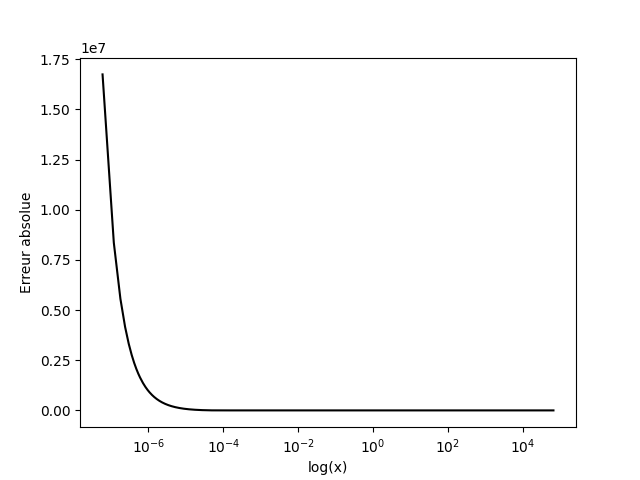
\includegraphics[width=12cm]{images/graph_inv.png}
    \label{fig:graph_inv.png}
\end{figure}\\
L'on observe alors que pour des valeurs de $x < 10^{-4}$, l'approximation n'est pas fiable.
\subsection{Calcul de fonctions trigonométriques}
Les méthodes d'approximation de fonctions trigonométriques sont variées, celle expliquée ci-dessous n'a pas tant été choisie pour son efficacité que pour son élégance et simplicité. Elle repose sur cette observation:
Remarquons que pour l'instant les seules fonctions que notre machine peut évaluer sont celles uniquement composées des 4 opérations élémentaires, dont des polynômes. Pour cette raison l'évaluation des fonctions trigonométriques parait impossible. Il sera alors utile de définir un outil pour convertir les fonctions désirées en polynômes, qui sont eux évaluables.
\subsubsection{Séries de Taylor}
Les séries de Taylor sont un outil puissant pour approximer les fonctions avec des polynômes. Admettons que l'on aie une fonction $f(x)$ et que l'on veuille un polynôme $P_n(x)$ qui approxime $f(x)$ autour de $a$. C'est a dire que plus $x$ s'éloigne de $a$, plus $P_n(x)$ s'éloigne de $f(x)$. Soit,
$$P_n(x) = c_0 + c_1(x-a) + c_2(x-a)^2+\cdot\cdot\cdot+c_n(x-a)^n.$$
Les coefficients $c_0, \cdot\cdot\cdot,c_n$ restent alors à déterminer.
Il parait intuitif que $P_n(a)$ devrait être égal à $f(a)$. Puisque $P_n(a) = c_0$, on en déduit $c_0=f(a)$. Ensuite, en continuant avec intuition, on décide que $P_n'(a) = f'(a)$. Et plus généralement $P_n^{(k)}(a) = f^{(k)}(a)$ pour tout $k\le n$, ou $f^{(k)}(x)$ désigne la $k$-ième dérivée de $f(x)$. En dérivant $k$ fois $P_n(x)$ on obtient
$$
P_n^{(k)}(x) = c_kk!+c_{k+1}(k+1)!(x-a)+\cdot\cdot\cdot+c_n\frac{n!}{(n-k)!}(x-a)^{n-k}.
$$
Alors $P_n^{(k)}(a) = c_kk!\;$, soit $c_k = \frac{f^{(k)}(a)}{k!}$.\\
Donc
$$P_n(x) = f(a) + f'(a)(x-a) + \frac{f''(a)}{2!}(x-a)^2+\cdot\cdot\cdot+\frac{f^{(n)}(a)}{n!}(x-a)^n.$$
Plus $n$ est grand, plus l'approximation est bonne.
On alors
$$f(x) = \sum_{k=1}^{\infty}\frac{f^{(k)}(a)}{k!}(x-a)^k.$$
La série associée ici à la fonction $f$ est appelée la série de Taylor de $f$ autour de $a$. Montrer qu'une fonction est en vérité égale à sa série de Taylor est un exercice plus compliqué et ne sera donc pas détaillé ici. Heureusement la grande partie des fonctions utilisées couramment le sont.
\subsubsection{Application des séries de Taylor pour le calcul de fonctions trigonométriques}
Maintenant que nous avons un outil pour convertir des fonctions en polynômes, essayons de l'appliquer sur les fonctions que nous voulons évaluer.
Par exemple, en prenant $f(x) = \sin(x)$ et $a = 0$ on obtient la série de Taylor de $\sin(x)$ autour de 0, 
$$\sin(x) = x - \frac{x^3}{3!} + \frac{x^5}{5!} - \frac{x^7}{7!} + \cdot\cdot\cdot.$$
Similairement, on peut obtenir la série de Taylor de $\cos(x)$ autour de 0,
$$\cos(x) = 1 - \frac{x^2}{2!} + \frac{x^4}{4!} - \frac{x^6}{6!} + \cdot\cdot\cdot.$$
En tronquant les séries ci-dessus à un nombre approprié de termes on obtient une expression qui est facilement évaluable par notre machine.
Vérifions maintenant graphiquement la précision de ces approximations.
\begin{center}
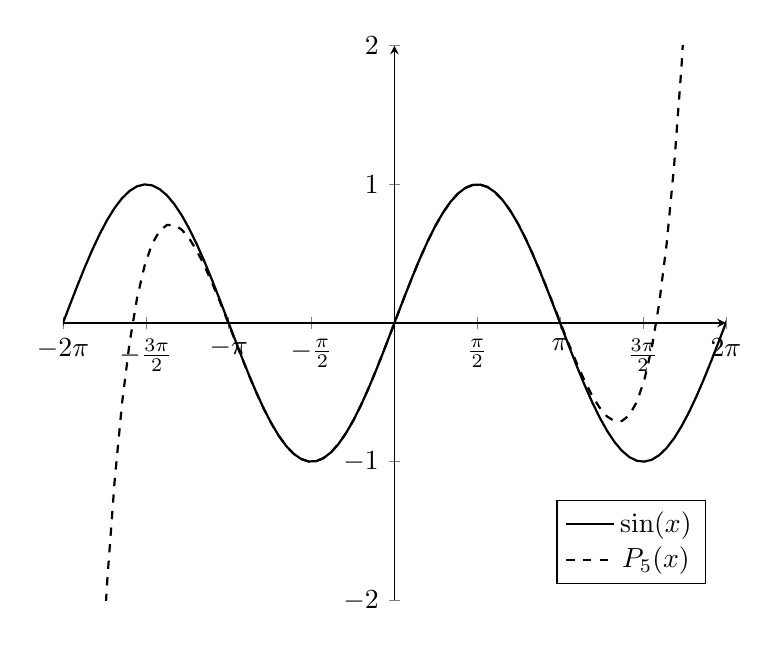
\begin{tikzpicture}[scale = 1]
\begin{axis}[xmin=-2*pi, xmax=2*pi, ymin=-2, ymax=2,
             axis lines=middle,
             xtick={-2*pi, -3*pi/2, -pi, -pi/2, 0, pi/2, pi, 3*pi/2, 2*pi},
             xticklabels={$-2\pi$, $-\frac{3\pi}{2}$, $-\pi$, $-\frac{\pi}{2}$, $0$, $\frac{\pi}{2}$, $\pi$, $\frac{3\pi}{2}$, $2\pi$},
             xticklabel style={anchor=north},
             legend pos=south east
             ]
\addplot[thick, domain=-7:7, color=black, samples=100]{sin(deg(x))};
\addplot[thick, domain=-7:7, dashed, color=black, samples=100]{x-(x^3)/3!+(x^5)/5!-(x^7)/7!+(x^9)/9!};
\addlegendentry{$\sin(x)$}
\addlegendentry{$P_5(x)$}
\end{axis}
\end{tikzpicture}
\end{center}
Comparons ici la fonction $\sin(x)$ et son approximation de Taylor tronquée à 5 termes, soit $x-\frac{x^3}{3!}+\frac{x^5}{5!}-\frac{x^7}{7!}+\frac{x^9}{9!}$. On s'arrête à 5 termes car le prochain impliquerait une multiplication par $\frac{1}{11!} \approx 2.5 \cdot 10^{-8}$ ce qui est inférieur a la valeur minimale représentable par nos floats ($\approx 6 \cdot 10^{-8})$. Intuitivement, il semblerait qu'il nous faut juste une approximation sur le segment $[0; 2\pi]$ et ensuite la périodicité de la fonction permettrait une approximation sur tout les réels. Pourtant, la meilleure approximation possible avec nos limitations physiques commence déjà à se dégrader autour de $x = \pi$. Pour remédier à ce problème, remarquons qu'on peut séparer la fonction en segments de longueur $\pi$ qui sont tous des symétries du premier segment $[-\frac{\pi}{2}; \frac{\pi}{2}]$ (sur lequel l'approximation semble plutôt rapprochée de la valeur exacte). C'est à dire que le premier segment encode toute l'information nécessaire pour représenter le reste de la fonction. Il faut alors un algorithme qui peut rabattre tout nombre dans sur son équivalent dans le segment $[-\frac{\pi}{2}; \frac{\pi}{2}]$. Soit, $x\rightarrow \theta$ avec $x \in \mathbb{R}$, $\sin(x) = \sin(\theta)$ et $\theta \in [-\frac{\pi}{2}; \frac{\pi}{2}]$. Ci-dessous est détaillé le pseudocode d'un tel algorithme:
\begin{algorithm}
\begin{algorithmic}[1]
\State $\theta \gets x\;\%\;2\pi$
\If{$x > \pi$}
    \State $\theta \gets \pi-\theta$
\EndIf
\\
\If{$|\theta| > \frac{\pi}{2}$}
    \If{$\theta < 0$}
        \State $\theta \gets \theta-\pi$
    \ElsIf{$\theta \ge 0$}
        \State $\theta \gets \pi-\theta$
    \EndIf
\EndIf
\end{algorithmic}
\end{algorithm}

Ici, l'opération \%, présente à la première ligne de l'algorithme, dénote l'opération tel que la relation $x\;\%\;y = z$ soit vraie si ces 3 conditions sont réunies: $x = z +ky$, $k \in \mathbb{Z}$ et $0\le z<y$. Cette opération est facilement calculable par notre machine en effectuant $z = x-y\cdot\text{trunc}(\frac{x}{y})$. Où $\text{trunc}(x)$ est la fonction qui associe à un réel $x$, sa partie entière. Ce qui est assez simple à faire avec un float.
Une fois $\theta$ trouvé, il suffit d'évaluer la série de Taylor en $\theta$.
Pour approximer $\cos(x)$ on utilise une méthode similaire, mais puisque $\cos(x)$ est positif sur le segment $[-\frac{\pi}{2}; \frac{\pi}{2}]$, il n'existe pas un $\theta$ compris dans ce segment tel que $\cos(x) = cos(\theta),\;\forall x \in \mathbb{R}.$ On peut en revanche trouver $\theta$, tel que $|\cos(x)| = cos(\theta)$, et le signe du résultat final, qu'on applique au résultat obtenu après l'évaluation de la série.
\subsubsection{Implémentation et résultats} 
Lors de l'implémentation, on remarque que le facteur limitant de la précision est l'opération \%, présente à la première ligne de l'algorithme. Pour cette raison une erreur absolue maximale $< 0.01$, n'est que garantie pour $x<34$. Mais puisqu'en pratique l'on calcule rarement le sinus ou le cosinus d'un nombre plus grand que $2\pi$, nous allons utiliser les bornes $-2\pi$ et $2\pi$ pour le calcul de l'erreur absolue moyenne. En procèdent de la même manière que précédemment pour la fonction inverse, on obtient, pour sinus, une erreur absolue moyenne de $\Bar{r}\approx 0.001$ et pour cosinus, une erreur absolue moyenne de $\Bar{r}\approx0.0008$.
\newpage
En traçant, pour sinus, l'erreur absolue sur l'intervalle $[0;2\pi]$, on obtient le graphique ci-dessous:
\begin{figure}[htp]
    \centering
    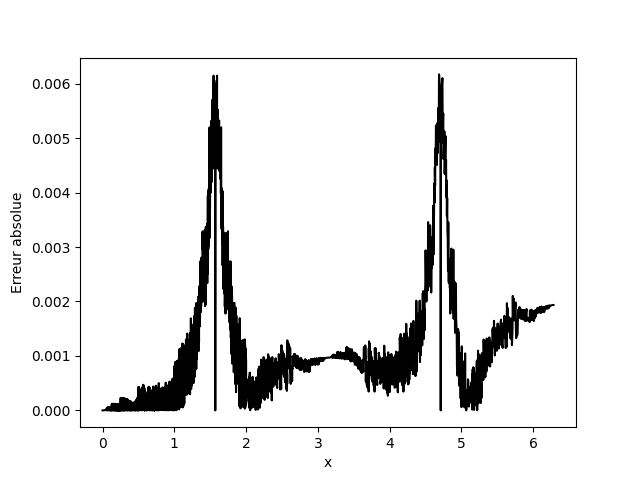
\includegraphics[width=12cm]{images/graph_sin.png}
    \label{fig:graph_sin.png}
\end{figure}\\
Soit, l'erreur est maximale autour de $x=\frac{\pi}{2}$ et $x=\frac{3\pi}{2}$. Ceci fait sens puisque ces points se trouvent aux extrémités des segments définis plus tôt et que la série de Taylor s'éloigne de la valeur exacte aux extrémités. De même pour l'approximation de la fonction cosinus.
\section{Calcul de décimales de pi}
\subsection{Méthode}
En utilisant la représentation float, la meilleur approximation possible de $\pi$ est égale à 3.140625. Alors, essayer de calculer un maximum de décimales de $\pi$ sous la forme d'un float est un exercice un peu décevant. Heureusement il existe des algorithmes qui ne travaillent que sur des entiers, et qui produisent, itérativement, des décimales de $\pi$. L'algorithme utilisé ici, découvert par Rabinowitz et Wagon en 1995 \cite{rabinowitz1995spigot}, est lui même basé sur un autre algorithme pour calculer les décimales de $e$, découvert par Sale en 1968 \cite{sale1968e} que nous allons détailler en premier afin de mieux comprendre celui pour $\pi$. Cet algorithme se base sur la somme infinie ci-dessous.
$$
e = \frac{1}{0!}+\frac{1}{1!}+\frac{1}{2!}+\frac{1}{3!}+\frac{1}{4!}+\frac{1}{5!}\cdot\cdot\cdot
$$
Cette série peut être notamment obtenue en évaluant la série de Taylor de $e^x$ autour de 0, en $x = 1$.
On peut ensuite réécrire cette série sous la forme
$$
e = 1+1\Bigl(1+\frac{1}{2}\Bigl(1+\frac{1}{3}\Bigl(1+\frac{1}{4}\Bigl(1+\frac{1}{5}\Bigl(1+\cdot\cdot\cdot\Bigr)\Bigr)\Bigr)\Bigr)\Bigr)
.$$
En tronquant, au besoin, le nombre de termes on obtient une approximation pour $e$.
Prenons par exemple cette approximation:
\begin{align*}  
e &\approx 1+1\Bigl(1+\frac{1}{2}\Bigl(1+\frac{1}{3}\Bigl(1+\frac{1}{4}\Bigl(1+\frac{1}{5}\Bigl(1\Bigr)\Bigr)\Bigr)\Bigr)\Bigr)\\
&\approx 2+\frac{1}{2}\Bigl(1+\frac{1}{3}\Bigl(1+\frac{1}{4}\Bigl(1+\frac{1}{5}\Bigl(1\Bigr)\Bigr)\Bigr)\Bigr)
\end{align*}

Remarquons ensuite que la partie fractionnelle de l'approximation, sous cette forme, est
$$
\frac{1}{2}\Bigl(1+\frac{1}{3}\Bigl(1+\frac{1}{4}\Bigl(1+\frac{1}{5}\Bigl(1\Bigr)\Bigr)\Bigr)\Bigr)
$$
et que donc la partie entière est 2.
Pour trouver la prochaine décimale, il suffit de multiplier la partie fractionnelle par 10, et de prendre sa partie entière. On a alors
$$
\frac{1}{2}\Bigl(10+\frac{1}{3}\Bigl(10+\frac{1}{4}\Bigl(10+\frac{1}{5}\Bigl(10\Bigr)\Bigr)\Bigr)\Bigr)
$$
$$
=7+\frac{1}{2}\Bigl(0+\frac{1}{3}\Bigl(1+\frac{1}{4}\Bigl(0+\frac{1}{5}\Bigl(0\Bigr)\Bigr)\Bigr)\Bigr).
$$
La partie entière est donc de 7. En répétant l'opération sur la partie fractionnelle, l'on peut obtenir la prochaine décimale et ainsi de suite. Cet algorithme est très simple et n'opère que sur des nombres entiers. Essayons maintenant d'appliquer une méthode similaire pour les décimales de $\pi$.
Premièrement il nous faut une représentation de $\pi$ propice a cet algorithme. Celle que nous allons utiliser découle du produit de Wallis pour $\pi$.\footnote{La dérivation, dépassant le cadre de ce travail, n'est pas détaillée ici.} 
$$
\frac{\pi}{2} = \sum_{k=1}^{\infty}\frac{k!}{(2k+1)!!}
$$
ou $(2k+1)!!$ dénote le produit des entiers impairs de 1 a $2k+1$, $(2k+1)!! = 1\cdot3\cdot5\cdot\cdot\cdot (2k+1)$. 
On en déduit alors une représentation propice a l'algorithme.
\begin{align*}
\frac{\pi}{2} &= 1 + \frac{1}{3} + \frac{1\cdot2}{3\cdot5} +  \frac{1\cdot2\cdot3}{3\cdot5\cdot7} + \frac{1\cdot2\cdot3\cdot4}{3\cdot5\cdot7\cdot9} + \cdot\cdot\cdot\\
 &= 1 + \frac{1}{3}\Bigl(1+\frac{2}{5}\Bigl(1+\frac{3}{7}\Bigl(1+\frac{4}{9}\Bigl(1+\cdot\cdot\cdot\Bigr)\Bigr)\Bigr)\Bigr)\\
 \pi &= 2 + \frac{1}{3}\Bigl(2+\frac{2}{5}\Bigl(2+\frac{3}{7}\Bigl(2+\frac{4}{9}\Bigl(2+\cdot\cdot\cdot\Bigr)\Bigr)\Bigr)\Bigr).
\end{align*}
Contrairement à l'algorithme pour $e$, la partie entière de $\pi$ n'est pas simplement donnée par le premier terme, car le deuxième terme n'est pas forcement inférieur à 1. Pour cette raison, quand une décimale est calculée il faut la garder en mémoire pour vérifier que la prochaine décimale n'est pas un 10. Dans quel cas on ajoute 1 à la décimale précédemment stockée. Opérons maintenant de la même manière que pour calculer les décimales de $e$:
$$
\pi \approx 2 + \frac{1}{3}\Bigl(2+\frac{2}{5}\Bigl(2+\frac{3}{7}\Bigl(2+\frac{4}{9}\Bigl(2\Bigr)\Bigr)\Bigr)\Bigr)
$$
On stocke donc le 2 et l'on garde que le deuxième terme qu'on multiplie par 10.
$$
\frac{1}{3}\Bigl(20+\frac{2}{5}\Bigl(20+\frac{3}{7}\Bigl(20+\frac{4}{9}\Bigl(20\Bigr)\Bigr)\Bigr)\Bigr)
$$
$$
=\frac{1}{3}\Bigl(20+\frac{2}{5}\Bigl(20+\frac{3}{7}\Bigl(20+\frac{4}{9}\Bigl(2\cdot9 + 2\Bigr)\Bigr)\Bigr)\Bigr)
$$
$$
=\frac{1}{3}\Bigl(20+\frac{2}{5}\Bigl(20+\frac{3}{7}\Bigl(20+2\cdot4+\frac{4}{9}\Bigl(2\Bigr)\Bigr)\Bigr)\Bigr)
$$
$$
=\frac{1}{3}\Bigl(20+\frac{2}{5}\Bigl(20+\frac{3}{7}\Bigl(28+\frac{4}{9}\Bigl(2\Bigr)\Bigr)\Bigr)\Bigr)
$$
En continuant de cette manière, de la droite vers la gauche on obtient:
$$
10 + \frac{1}{3}\Bigl(2+\frac{2}{5}\Bigl(2+\frac{3}{7}\Bigl(0+\frac{4}{9}\Bigl(2\Bigr)\Bigr)\Bigr)\Bigr)
$$
Puisque la prochaine décimale est un 10 on en déduit donc que la première décimale (ou chiffre dans ce cas) de $\pi$ est un 3. En continuant de la même manière l'on peut aisément calculer le reste des décimales offertes par cette approximation. Cette explication omet, par volonté de simplifier, certains aspects. Mais l'idée générale reste la même. 
\subsection{Implémentation et résultats}
Pour implémenter cet algorithme on représente l'approximation comme une liste remplie de 2, sur laquelle il est facile de manipuler chaque entrée en fonction de sa position dans la liste. Il parait intuitif que plus la liste est grande, meilleure l'approximation sera et donc plus on aura de décimales correctes. Puisque dans notre cas l'espace de mémoire est une contrainte plutôt importante il sera important d'écrire un programme le plus court possible, de sorte à pouvoir utiliser le reste de la mémoire pour une liste de taille maximale. Dans notre cas il a été possible d'écrire un programme assez court pour que la liste aie 32'485 entrées de 16 bits. En effectuant 10'000 itérations, on obtient alors 10'000 décimales de $\pi$. Après avoir comparé les décimales obtenues avec les décimales correctes, on s'aperçoit que nos décimales ne diffèrent qu'à partir de la 9724-ème décimale. Soit, notre processeur a correctement calculé 9723 décimales de $\pi$. Notons que ce résultat, bien qu'impressionnant, n'a absolument aucune utilité pratique, puisque seulement 38 décimales suffisent pour calculer le périmètre d'un disque de la taille de l'univers observable avec une précision de l'ordre du rayon d'un atome d'hydrogène. \cite{yates_2024}
\section{Conclusion}
Mieux comprendre les outils qu'on utilise, permet de les exploiter au maximum de leur capacités. Ce travail a exploré quelques-uns des concepts fondamentaux présents dans tous les ordinateurs modernes. En effet, bien que notre machine soit beaucoup plus simple que celles d'aujourd'hui, les bases restent les mêmes. Cependant, cette simplicité entraîne une précision inférieure au standards modernes. Les limitations physiques de notre machine étaient l'obstacle majeur qu'il a fallu au mieux contourner. Une autre limitation majeure, qui n'a pas été traitée dans ce travail, est celle du temps d’exécution. En effet, avec un processeur émulé il est difficile de savoir combien de temps un programme aurait prit si il avait exécuté par une vraie machine. En tout, ce travail montre que bien que ça puisse parfois paraître être le cas, rien en informatique est de l'ordre de la magie. Tout peut être ramené à une poignée d'opérations simples réalisables par n'importe qui.
\vspace{2cm}
\begin{figure}[htp]
    \centering
    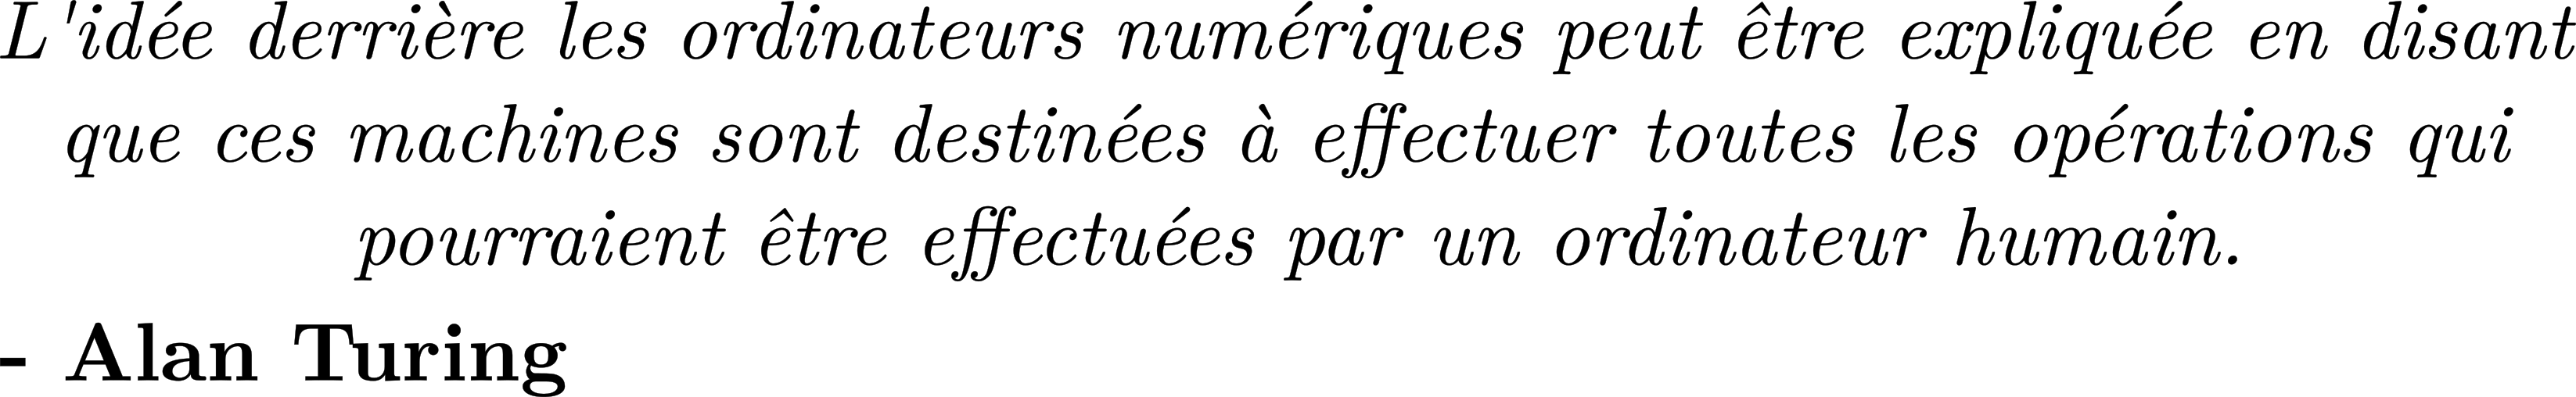
\includegraphics[width=12cm]{images/quote.png}
    \label{fig:quote}
\end{figure}

\newpage
\printbibliography

\end{document}
